\section{Preconditioners}
\label{sec:precon}

Most of the solvers in \nekpp, including the incompressible Navier-Stokes
equations, rely on the solution of a Helmholtz equation,
%
\begin{equation}
  \nabla^{2}u(\mathbf{x})+\lambda u(\mathbf{x})=f(\mathbf{x}),
  \label{eq:precon:helm}
\end{equation}
%
an elliptic boundary value problem, at every time-step, where $u$ is defined on
a domain $\Omega$ of $N_{\mathrm{el}}$ non-overlapping elements. In this
section, we outline the preconditioners which are implemented in \nekpp. Whilst
some of the preconditioners are generic, many are especially designed for the
\emph{modified} basis only.

\subsection{Mathematical formulation}

The standard spectral/$hp$ approach to discretise \eqref{eq:precon:helm} starts
with an expansion in terms of the elemental modes:
%
\begin{equation}
  u^{\delta}(\mathbf{x})=\sum_{n=0}^{N_{\mathrm{dof}}-1}\hat{u}_n
  \Phi_n(\mathbf{x})=\sum_{e=1}^{{N_{\mathrm{el}}}}
  \sum_{n=0}^{N^{e}_m-1}\hat{u}_n^e\phi_n^e(\mathbf{x})
  \label{eq:precon:disc}
\end{equation}
%
where $N_{\mathrm{el}}$ is the number of elements, $N^{e}_m$ is the number of
local expansion modes within the element $\Omega^e$, $\phi_n^e(\mathbf{x})$ is
the $n^{\mathrm{th}}$ local expansion mode within the element $\Omega^e$,
$\hat{u}_n^e$ is the $n^{\mathrm{th}}$ local expansion coefficient within the
element $\Omega^e$. Approximating our solution by~\eqref{eq:precon:disc}, we
adopt a Galerkin discretisation of equation~\eqref{eq:precon:helm} where for an
appropriate test space $V^\delta$ we find an approximate solution
$\mathbf{u}^{\delta} \in V^{\delta}$ such that
%
\[
\mathcal L \left({v, u}\right) = \int_{\Omega}\nabla v^{\delta} \cdot \nabla
u^{\delta} + \lambda v^{\delta} u^{\delta} d \mathbf{x} = \int_{\Omega}
v^{\delta} f d\mathbf{x} \quad \forall v^{\delta} \in V^{\delta}
\]
%
This can be formulated in matrix terms as
%
\[
\mathbf{H}\hat{\mathbf{u}} = \mathbf{f}
\]
%
where $\mathbf{H}$ represents the Helmholtz matrix, $\hat{\mathbf{u}}$ are the
unknown global coefficients and $\mathbf{f}$ the inner product the expansion
basis with the forcing function.

\subsubsection{$C^0$ formulation}

We first consider the $C^0$ (i.e. continuous Galerkin) formulation. The
spectral/$hp$ expansion basis is obtained by considering interior modes, which
have support in the interior of the element, separately from boundary modes
which are non-zero on the boundary of the element. We align the boundary modes
across the interface of the elements to obtain a continuous global solution. The
boundary modes can be further decomposed into vertex, edge and face modes,
defined as follows:

\begin{itemize}
  \item vertex modes have support on a single vertex and the three adjacent
  edges and faces as well as the interior of the element;
  \item edge modes have support on a single edge and two adjacent faces as well
  as the interior of the element; 
  \item face modes have support on a single face and the interior of the
  element.
\end{itemize}

When the discretisation is continuous, this strong coupling between vertices,
edges and faces leads to a matrix of high condition number $\kappa$. Our aim is
to reduce this condition number by applying specialised
preconditioners. Utilising the above mentioned decomposition, we can write the
matrix equation as:
%
\[
\left[\begin{array}{cc}
  \mathbf{H}_{bb} & \mathbf{H}_{bi}\\
  \mathbf{H}_{ib} & \mathbf{H}_{ii}
  \end{array}\right]
\left[ \begin{array}{c}
\hat{\mathbf{u}}_{b}\\
\hat{\mathbf{u}}_{i}\\
\end{array}\right] =
\left[ \begin{array}{c}
\hat{\mathbf{f}}_{b}\\
\hat{\mathbf{f}}_{i}\\
\end{array}\right]
\]
%
where the subscripts $b$ and $i$ denote the boundary and interior degrees of
freedom respectively. This system then can be statically condensed allowing us
to solve for the boundary and interior degrees of freedom in a decoupled
manor. The statically condensed matrix is given by
%
\[
\left[\begin{array}{cc}
  \mathbf{H}_{bb}-\mathbf{H}_{bi} \mathbf{H}_{ii}^{-1} \mathbf{H}_{ib} & 0\\
  \mathbf{H}_{ib} & \mathbf{H}_{ii}
  \end{array}\right]
\left[ \begin{array}{c}
\hat{\mathbf{u}}_{b}\\
\hat{\mathbf{u}}_{i}\\
\end{array}\right] =
\left[ \begin{array}{c}
\hat{\mathbf{f}}_{b}-\mathbf{H}_{bi} \mathbf{H}_{ii}^{-1}\hat{\mathbf{f}}_{i}\\
\hat{\mathbf{f}}_{i}\\
\end{array}\right]
\]
%
This is highly advantageous since by definition of our interior expansion this
vanishes on the boundary, and so $\mathbf{H}_{ii}$ is block diagonal and thus
can be easily inverted. The above sub-structuring has reduced our problem to
solving the boundary problem:
%
\[
\mathbf{S}_{1}\hat{\mathbf{u}} = \hat{\mathbf{f}}_{1}
\]
%
where
$\mathbf{S_{1}}=\mathbf{H}_{bb}-\mathbf{H}_{bi} \mathbf{H}_{ii}^{-1}
\mathbf{H}_{ib}$
and
$\hat{\mathbf{f}}_{1}=\hat{\mathbf{f}}_{b}-\mathbf{H}_{bi}
\mathbf{H}_{ii}^{-1}\hat{\mathbf{f}}_{i}$.
Although this new system typically has better convergence properties (i.e lower
$\kappa$), the system is still ill-conditioned, leading to a convergence rate of
the conjugate gradient (CG) routine that is prohibitively slow. For this reason
we need to precondition $\mathbf{S}_1$. To do this we solve an equivalent
system of the form:
%
\[
\mathbf{M}^{-1}\left(\mathbf{S}_{1} \hat{\mathbf{u}} - \hat{\mathbf{f}}_{1} \right) = 0
\]
%
where the preconditioning matrix $\mathbf{M}$ is such that
$\kappa\left(\mathbf{M}^{-1} \mathbf{S}_{1}\right)$ is less than
$\kappa\left(\mathbf{S}_{1}\right)$ and speeds up the convergence rate. Within
the conjugate gradient routine the same preconditioner $\mathbf{M}$ is applied
to the residual vector $\hat{\mathbf{r}}_{k+1}$ of the CG routine every
iteration:
%
\[
\hat{\mathbf{z}}_{k+1}=\mathbf{M}^{-1}\hat{\mathbf{r}}_{k+1}.
\]
%

\subsubsection{HDG formulation}

When utilising a hybridizable discontinuous Galerkin formulation, we perform a
static condensation approach but in a discontinuous framework, which for brevity
we omit here. However, we still obtain a matrix equation of the form
%
\[
\mathbf{\Lambda}\hat{\mathbf{u}} = \hat{\mathbf{f}}.
\]
%
where $\mathbf{\Lambda}$ represents an operator which projects the solution of
each face back onto the three-dimensional element or edge onto the
two-dimensional element. In this setting then, $\hat{\mathbf{f}}$ consists of
degrees of freedom for each egde (in 2D) or face (in 3D). The overall system
does not, therefore, results in a weaker coupling between degrees of freedom,
but at the expense of a larger matrix system.

\subsection{Preconditioners}

Within the \nekpp framework a number of preconditioners are available to speed
up the convergence rate of the conjugate gradient routine. The table below
summarises each method, the dimensions of elements which are supported, and also
the discretisation type support which can either be continuous (CG) or
discontinuous (hybridizable DG).

\begin{center}
  \begin{tabular}{lll}
    \toprule
    \textbf{Name}  & \textbf{Dimensions} & \textbf{Discretisations} \\
    \midrule
    \inltt{Null}                              & All  & All \\
    \inltt{Diagonal}                          & All  & All \\
    \inltt{FullLinearSpace}                   & 2/3D & CG  \\
    \inltt{LowEnergyBlock}                    & 3D   & CG  \\
    \inltt{Block}                             & 2/3D & All \\
    \inltt{LOR}                             & 2/3D & CG \\
    \midrule
    \inltt{FullLinearSpaceWithDiagonal}       & All  & CG  \\
    \inltt{FullLinearSpaceWithLowEnergyBlock} & 2/3D & CG  \\
    \inltt{FullLinearSpaceWithBlock}          & 2/3D & CG  \\
    \bottomrule
  \end{tabular}
\end{center}

The default is the \inltt{Diagonal} preconditioner. The above preconditioners
are specified through the \inltt{Preconditioner} option of the
\inltt{SOLVERINFO} section in the session file. For example, to enable
\inltt{FullLinearSpace} one can use:

\begin{lstlisting}[style=XMLStyle]
  <I PROPERTY="Preconditioner" VALUE="FullLinearSpace" />
\end{lstlisting}

Alternatively one can have more control over different preconditioners for each
solution field by using the \inltt{GlobalSysSoln} section. For more details,
consult the user guide. The following sections specify the details for each
method.

\subsubsection{Diagonal}

Diagonal (or Jacobi) preconditioning is amongst the simplest preconditioning
strategies. In this scheme one takes the global matrix $\mathbf{H} = (h_{ij})$
and computes the diagonal terms $h_{ii}$. The preconditioner is then formed as a
diagonal matrix $\mathbf{M}^{-1} = (h_{ii}^{-1})$.

\subsubsection{Linear space}

The linear space (or coarse space) of the matrix system is that containing
degrees of freedom corresponding only to the vertex modes in the high-order
system. Preconditioning of this space is achieved by forming the matrix
corresponding to the coarse space and inverting it, so that
%
\[
\mathbf{M}^{-1} = (\mathbf{S}^{-1}_{1})_{vv}
\]
%
Since the mesh associated with higher order methods is relatively coarse
compared with traditional finite element discretisations, the linear space can
usually be directly inverted without memory issues. However such a methodology
can be prohibitive on large parallel systems, due to a bottleneck in
communication.

In \nekpp the inversion of the linear space present is handled using the
$XX^{T}$ library. $XX^{T}$ is a parallel direct solver for problems of the form
$\mathbf{A}\hat{\mathbf{x}} = \hat{\mathbf{b}}$ based around a sparse
factorisation of the inverse of $\mathbf{A}$. To precondition utilising this
methodology the linear sub-space is gathered from the expansion and the
preconditioned residual within the CG routine is determined by solving
%
\[
(\mathbf{S}_{1})_{vv}\hat{\mathbf{z}}=\hat{\mathbf{r}}
\]
%
The preconditioned residual $\hat{\mathbf{z}}$ is then scattered back to the
respective location in the global degrees of freedom.

\subsubsection{Block}

Block preconditioning of the $C^0$ continuous system is defined by the
following:
%
\[
\mathbf{M}^{-1}=\left[ \begin{array}{ccc}
(\mathbf{S}^{-1}_{1})_{vv} & 0 & 0 \\
0 & (\mathbf{S}^{-1}_{1})_{eb} & 0\\
0 & 0 & (\mathbf{S}^{-1}_{1})_{ef}\\
 \end{array} \right]
\]
%
where $\mathrm{diag}[(\mathbf{S}_{1})_{vv}]$ is the diagonal of the vertex
modes, $(\mathbf{S}_{1})_{eb}$ and $(\mathbf{S}_{1})_{fb}$ are block diagonal
matrices corresponding to coupling of an edge (or face) with itself i.e ignoring
the coupling to other edges and faces. This preconditioner is best suited for
two dimensional problems.

In the HDG system, we take the block corresponding to each face and invert
it. Each of these inverse blocks then forms one of the diagonal components of
the block matrix $\mathbf{M}^{-1}$.

Applied to the full matrix system $\mathbf{H}$, the preconditioner additionally includes the inverse of the interior modes $\mathbf{H}_{ii}$ and is defined by:
%
\[
\mathbf{M}^{-1}=\left[\begin{array}{cccc}
(\mathbf{H_{bb}})^{-1}_{vv} & 0 & 0 & 0 \\
0 & (\mathbf{H_{bb}})^{-1}_{eb} & 0 & 0 \\
0 & 0 & (\mathbf{H_{bb}})^{-1}_{fb} & 0 \\
0 & 0 & 0 & (\mathbf{H}_{ii})^{-1}
\end{array}\right]
\]
%

\subsection{Low energy}

Low energy basis preconditioning follows the methodology proposed by Sherwin \&
Casarin. In this method a new basis is numerically constructed from the original
basis which allows the Schur complement matrix to be preconditioned using a
block preconditioner. The method is outlined briefly in the following.

Elementally the local approximation $\mathbf{u}^{\delta}$ can be expressed as
different expansions lying in the same discrete space $V^{\delta}$
%
\[
\mathbf{u}^{\delta}(\mathbf{x})=\sum_{i}^{\dim(V^{\delta})}\hat{u}_{1i}\phi_{1i}(x)
= \sum_{i}^{\dim(V^{\delta})}\hat{u}_{2i}\phi_{2j}(x)
\]
%
Since both expansions lie in the same space it's possible to express one basis
in terms of the other via a transformation, i.e.
%
\[
\phi_{2}=\mathbf{C}\phi_{1} \implies \hat{\mathbf{u}}_{1}=C^{T}\hat{\mathbf{u}}_{2}
\]
%
Applying this to the Helmholtz operator it is possible to show that,
%
\[
\mathbf{H}_{2}=\mathbf{C}\mathbf{H}_{1}\mathbf{C}^{T}
\]
%
For sub-structured matrices ($\mathbf{S}$) the transformation matrix
($\mathbf{C}$) becomes:
%
\[
\mathbf{C}=\left[ \begin{array}{cc}
\mathbf{R} & 0\\
0 & \mathbf{I}
 \end{array} \right]
\]
%
Hence the transformation in terms of the Schur complement matrices is:
%
\[
\mathbf{S}_{2}=\mathbf{R}\mathbf{S}_{1}\mathbf{R}^{T}
\]
%
Typically the choice of expansion basis $\phi_{1}$ can lead to a Helmholtz
matrix that has undesirable properties i.e poor condition number. By choosing a
suitable transformation matrix $\mathbf{C}$ it is possible to construct a new
basis, numerically, that is amenable to block diagonal preconditioning.
%
\[
\mathbf{S}_{1}=\left[ \begin{array}{ccc}
\mathbf{S}_{vv} & \mathbf{S}_{ve} & \mathbf{S}_{vf}\\
\mathbf{S}^{T}_{ve}& \mathbf{S}_{ee} & \mathbf{S}_{ef} \\
\mathbf{S}^{T}_{vf} & \mathbf{S}^{T}_{ef} & \mathbf{S}_{ff} \end{array} \right] =\left[ \begin{array}{cc}
\mathbf{S}_{vv} & \mathbf{S}_{v,ef} \\
\mathbf{S}^{T}_{v,ef} & \mathbf{S}_{ef,ef} \end{array} \right]
\]
%
Applying the transformation
$\mathbf{S}_{2}=\mathbf{R} \mathbf{S}_{1} \mathbf{R}^{T}$ leads to the following
matrix
%
\[
\mathbf{S}_{2}=\left[ \begin{array}{cc}
\mathbf{S}_{vv}+\mathbf{R}_{v}\mathbf{S}^{T}_{v,ef}+\mathbf{S}_{v,ef}\mathbf{R}^{T}_{v}+\mathbf{R}_{v}\mathbf{S}_{ef,ef}\mathbf{R}^{T}_{v} & [\mathbf{S}_{v,ef}+\mathbf{R}_{v}\mathbf{S}_{ef,ef}]\mathbf{A}^{T} \\
\mathbf{A}[\mathbf{S}^{T}_{v,ef}+\mathbf{S}_{ef,ef}\mathbf{R}^{T}_{v}] & \mathbf{A}\mathbf{S}_{ef,ef}\mathbf{A}^{T} \end{array} \right]
\]
%
where $\mathbf{A}\mathbf{S}_{ef,ef}\mathbf{A}^{T}$ is given by
%
\[
\mathbf{A}\mathbf{S}_{ef,ef}\mathbf{A}^{T}=\left[ \begin{array}{cc}
\mathbf{S}_{ee}+\mathbf{R}_{ef}\mathbf{S}^{T}_{ef}+\mathbf{S}_{ef}\mathbf{R}^{T}_{ef}+\mathbf{R}_{ef}\mathbf{S}_{ff}\mathbf{R}^{T}_{ef} & \mathbf{S}_{ef}+\mathbf{R}_{ef}\mathbf{S}_{ff}\\
\mathbf{S}^{T}_{ef}+\mathbf{S}_{ff}\mathbf{R}^{T}_{ef} & \mathbf{S}_{ff}
 \end{array} \right]
\]
%
To orthogonalise the vertex-edge and vertex-face modes, it can be seen from the
above that
%
\[
\mathbf{R}^{T}_{ef}=-\mathbf{S}^{-1}_{ff}\mathbf{S}^{T}_{ef}
\]
%
and for the edge-face modes:
%
\[
\mathbf{R}^{T}_{v}=-\mathbf{S}^{-1}_{ef,ef}\mathbf{S}^{T}_{v,ef}
\]
%
Here it is important to consider the form of the expansion basis since the
presence of $\mathbf{S}^{-1}_{ff}$ will lead to a new basis which has support on
all other faces; this is problematic when creating a $C^{0}$ continuous global
basis.  To circumvent this problem when forming the new basis, the decoupling is
only performed between a specific edge and the two adjacent faces in a symmetric
standard region. Since the decoupling is performed in a rotationally symmetric
standard region the basis does not take into account the Jacobian mapping
between the local element and global coordinates, hence the final expansion will
not be completely orthogonal.

The low energy basis creates a Schur complement matrix that although it is not
completely orthogonal can be spectrally approximated by its block diagonal
contribution. The final form of the preconditioner is:
%
\[
\mathbf{M}^{-1}=\left[ \begin{array}{ccc}
\mathrm{diag}[(\mathbf{S}_{2})_{vv}] & 0 & 0 \\
0 & (\mathbf{S}_{2})_{eb} & 0\\
0 & 0 & (\mathbf{S}_{2})_{fb}\\
 \end{array} \right]^{-1}
\]
%
where $\mathrm{diag}[(\mathbf{S}_{2})_{vv}]$ is the diagonal of the vertex
modes, $(\mathbf{S}_{2})_{eb}$ and $(\mathbf{S}_{2})_{fb}$ are block diagonal
matrices corresponding to coupling of an edge (or face) with itself i.e ignoring
the coupling to other edges and faces.

\subsection{Lower-order Refined (LOR) preconditioner}

For the construction of the LOR preconditioner, the global matrix $\mathbf{H}$ is interpolated from the higher-order spectral/\textit{hp} discretisation to its corresponding low-order (\textit{P}=1) ``refined" finite element discretisation $\mathbf{H}_{L}$. The conceptual representation of this conversion is seen in Fig.~\ref{fig:LOR_concept}, where the LOR mesh on the right is a sub-structured grid of collocated Gauss-Lobatto-Legendre (GLL) nodal points. The application of the preconditioning matrix $\mathbf{M}$ is then formulated as $\mathbf{M}^{-1} = \mathbf{H}_L^{-1}$.
\begin{figure}[!htbp]
    \centering
    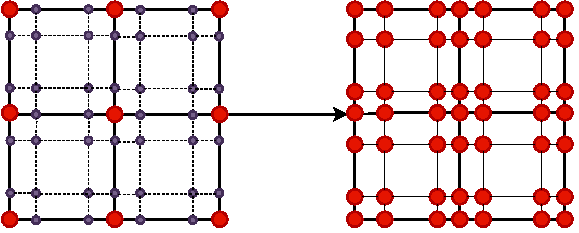
\includegraphics[width=0.4\textwidth]{img/LORpreconditioner.pdf}
    \caption{Representation of converting a higher-order finite element grid at \textit{P}=3 to its lower-order \textit{P}=1 equivalent for the LOR preconditioner. The red dots represent the points on the linear mesh, and the purple dots represent the quadrature points within a linear element. The resulting LOR mesh only contains linear DOF. The spacing of the linear DOF for the LOR mesh here is done in a GLL manner, the same as that of the higher-order element.}
    \label{fig:LOR_concept}
\end{figure}

For the high-order discretisation $\mathbf{H}$, every internal DOF is coupled with every other DOF in an element. The conversion to the LOR space $\mathbf{H}_{L}$ increases the sparsity as now the DOF are only connected to their immediate neighbours. The difference in connectivity between the two discretisations is further accentuated in mathematical operators, even if the number of DOF is the same (as seen in Fig.~\ref{fig:LOR_concept}). Thus, the operators on the lower-order discretisation are cheaper to evaluate than their higher-order counterparts.

The generalised Vandemonde matrix $\mathcal{V}$ from Eqn.~\eqref{eqn:gen_Vandemonde} is used for the interpolation of the higher-order polynomial space to the collocated Lagrange basis in the LOR space. In matrix terms, this interpolation is expressed as, 
\begin{equation}
    \mathcal{V} \hat{\mathbf{f}} = \mathbf{f}
    \label{eqn:gen_Vandemonde}
\end{equation}
where, $\mathbf{f} [i] = f (\mathbf{\xi_{i}})$ is the known polynomial expansion, $ \mathcal{V} [i][j] = {\phi_{j}} (\mathbf{\xi_{i}})$ where $\phi_{j}$ is the chosen basis function and $\hat{\mathbf{f}} [j] = \hat{f} (\mathbf{\xi_{j}})$ are the unknown expansion coefficients. The unknown Lagrange polynomials are then found using  $\hat{\mathbf{f}} = \mathcal{V}^{-1} \mathbf{f}$. The interpolation basis works for any basis selection in the HO space, where the matrix $\mathcal{V}$ is appropriately constructed according to the choice of higher-order expansion basis \cite{karniadakis2005spectral}. The interpolation for the case of the nodal expansion corresponds to a collocation projection. In contrast, a modal expansion basis is more involved as the construction of $\mathcal{V}$ has to handle the change of basis. The interpolation step is applied to both the trial and test functions in the higher-order polynomial space, and the interpolated functions are then used to construct $\mathbf{H}_{L}$.

Fig.~\ref{fig:LOR_process} gives an overview of the Nektar++ LOR preconditioner algorithm. 
\begin{figure}[!htbp]
        \centering
        \begin{tikzpicture}
            \node[anchor=south west,inner sep=0] (image) at (0,0) {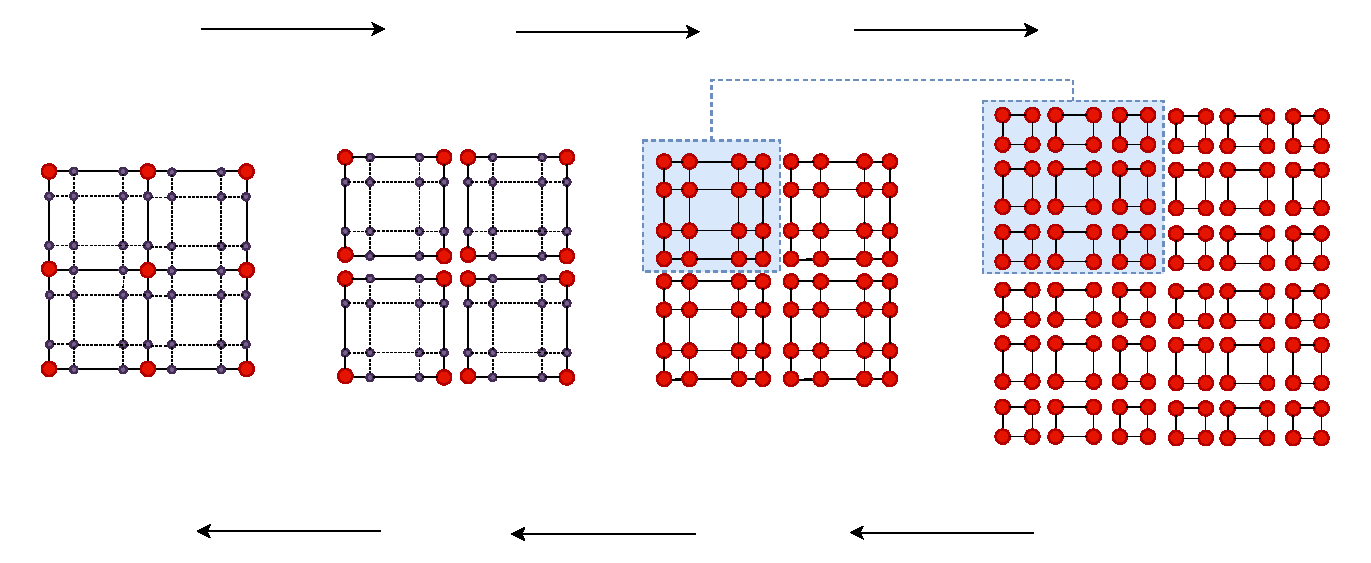
\includegraphics[width=\textwidth]{img/LOR_process_Nektar.drawio.pdf}};
            \node[below] at (1.6, 4.8) {Input $\hat{\mathbf{r}}$};
            \node[below] at (12.2, 1.2) {Solve LOR System};
            
            %top row annotations
            \node[below] at (3.0, 6.2) {\footnotesize Global to Local};
            % \node[below] at (2.2, 4.7) {$\hat{r}_{H,l} = \mathcal{A}_H \hat{r}_{H,g}$};
            \node[below] at (6.5, 6.2) {\footnotesize Change of basis: HO to LOR};
            % \node[below] at (5.2, 4.7) {$\hat{r}_{L,g} = \mathcal{V}^{-1} \hat{r}_{H,l}$};
            \node[below] at (10.0, 6.2) {\footnotesize Scatter};
            % \node[below] at (8.2, 4.7) {$\hat{r}_{L,l} = \mathcal{A}_{L} \hat{r}_{L,g}$};
            
            %bottom row annotations
            \node[below] at (3.0, 0.9) {\footnotesize Local to Global};
            % \node[below] at (2.2, 0.1) {$\hat{r}_{H,g} = \mathcal{A}_H^T \hat{r}_{H,l}$};
            \node[below] at (6.5, 0.9) {\footnotesize Change of basis: LOR to HO};
            % \node[below] at (5.2, 0.1) {$\hat{r}_{H,l} = \mathcal{V} \hat{r}_{L,g}$};
            \node[below] at (10.0, 0.9) {\footnotesize Gather};
            % \node[below] at (8.2, 0.1) {$\hat{r}_{L,g} = \mathcal{A}_{L}^{-1} \hat{r}_{L,l}$};
        \end{tikzpicture}
        \caption{Representation of the current algorithm for the LOR preconditioner. There are three major steps: a. The conversion to the LOR mesh (left to right), b. solving the LOR linear system and c. projecting the solution back to the HO mesh (right to left). This process takes place at every preconditioned iteration. }
        % $H$ is HO discretisation, $\mathcal{A}_H$ is the Assembly map in the HO space, $L$ is LOR discretisation, $\mathcal{A}_L$ is the Assembly map in the LOR space, $\mathcal{V}$ is the appropriate generalised Vandemonde matrix for interpolation from HO to LOR and vice versa, $g$, $l$ are global, local spaces.
        \label{fig:LOR_process}
\end{figure}

The following steps are done for the preconditioning:
\begin{itemize}
  \item The input to the LOR preconditioner code is the residual of the iterative solution $\hat{\mathbf{r}}$ at a given iteration (like all other preconditioners in Nektar++).
  \item The LOR space ($\mathbf{H}_L$) is generated at the \inltt{PreconditionerLOR::v\_BuildPreconditioner} step, using the \inltt{MeshGraph::LinearMeshGraph} method. This method has further setups to handle the LOR space for each element type (\inltt{LinMeshSetUp1DGeom}, \inltt{LinMeshSetUp2DGeom}, \inltt{LinMeshSetUpTetGeom}, \inltt{LinMeshSetUpPrismGeom}). A coefficient map (\inltt{m\_ho2lor}) is also generated during this step to handle the transformations between HO and LOR spaces and vice versa.
  \item Interpolation of the solution from the HO discretization to the LOR space is performed using an appropriately constructed generalized Vandermonde matrix $\mathcal{V}$, which depends on the choice of the higher-order expansion basis (MODIFIED or GLL\_LAGRANGE). This interpolation is managed by \inltt{MultiplyByBlockMatrix} operations in the \inltt{PreconditionerLOR::v\_DoPreconditioner} routine. Special keys (\inltt{eGLLToCoeffs} and \inltt{eEquiSpacedToCoeffs}) and their implementations are defined in the \inltt{ExpList} and \inltt{StdExpansion} classes to handle this process.
  \item After interpolating to the LOR space, the linear system is solved using an appropriate inner-iteration strategy. This is done using \inltt{m\_LORLinSys->SolveLinearSystem} within \inltt{PreconditionerLOR::v\_DoPreconditioner}.
  \item The solution from the LOR mesh is then mapped back to the HO space and subsequently transformed onto the original expansion basis by applying the inverse of the $\mathcal{V}$ matrix operation. Essentially, this reverses the steps taken before solving the LOR system.
  \item Appropriate scatter-gather transformations are handled using the assembly maps (\inltt{m\_ho2lor}) in both spaces.
\end{itemize}

\subsubsection{LOR spaces for different element types}

The choice of discretisation in the LOR space has a bearing on the conditioning properties of the LOR preconditioner. There are two options for the point distribution in the LOR space - equispaced and GLL distribution. The GLL distribution is consistent with the spectral equivalence of the HO-LOR spaces. Still, the former option is solely available to test the preconditioner performance for an equidistant point spacing. The default point distribution for the LOR preconditioner is GLL distribution. It can be activated using the property \inltt{LORPointDistribution}, with the options \inltt{GLL} and \inltt{Equispaced}.

There are two options to discretise the quadrilaterals in the LOR space in the Nektar++ implementation following the work of Canuto \cite{Canuto2009}, namely $\mathcal{Q}1$ and $\mathcal{P}1$ elements. The differences can be seen in Figure ~\ref{fig:P1vsQ1}, where for a given quadrilateral element at a fixed polynomial order the GLL points in the LOR space can either be formulated with $\mathcal{Q}1$ (quadrilateral) elements or $\mathcal{P}1$ (triangular) elements. 
\begin{figure}[!htbp]
    \centering
    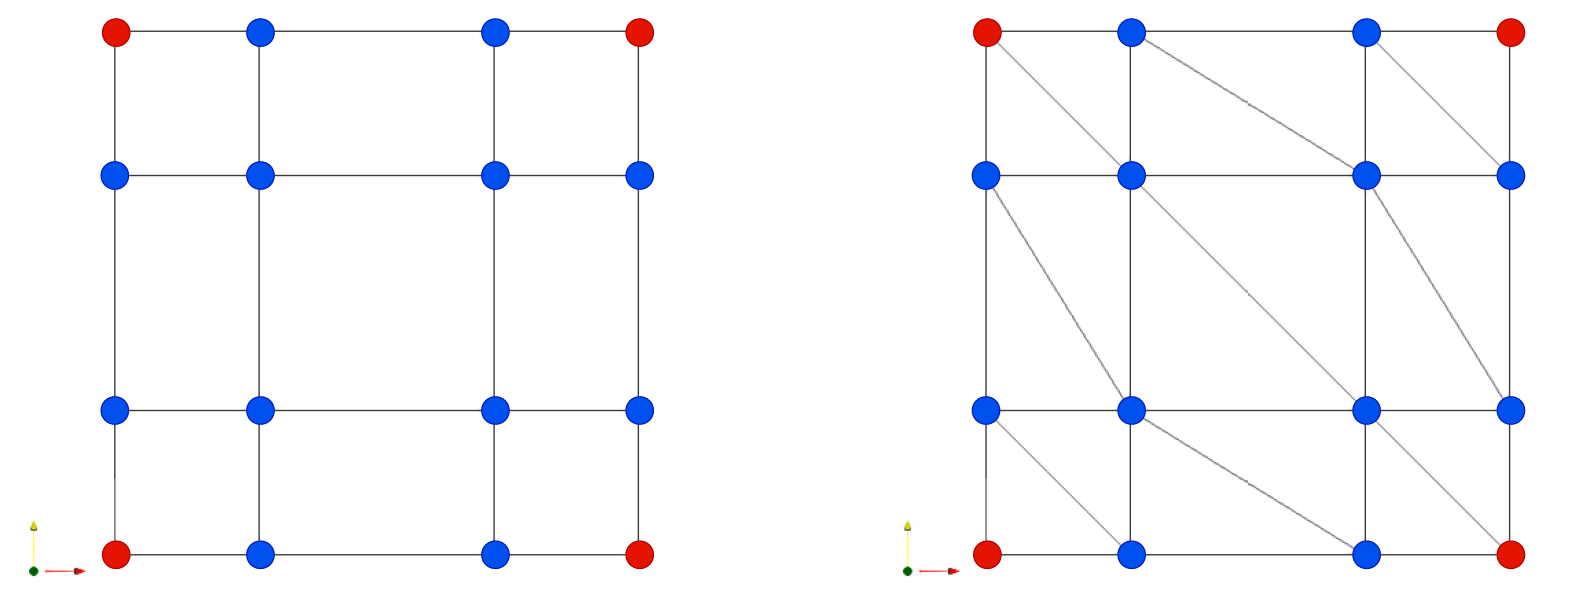
\includegraphics[width=0.5\textwidth]{img/P1vsQ1_crop.png} 
    \caption{Available options for the LOR grids for the quadrilateral elements in 2D. The red dots correspond to the original HO element, and the blue dots are the GLL points in the LOR for \textit{P}=3. Left: $\mathcal{Q}1$ configuration, Right: $\mathcal{P}1$ configuration.}
    \label{fig:P1vsQ1}
\end{figure}
Notice that there can be many possible orientations for $\mathcal{P}1$ elements, and the choice in Figure ~\ref{fig:P1vsQ1} is one such possibility. There are no such options for triangular elements in the LOR space as they can only be discretised in further smaller P1 elements.
It can be activated using the property \inltt{LORSimplex}, with the options \inltt{False} for $\mathcal{Q}1$ (default) and \inltt{True} for $\mathcal{P}1$.

\begin{figure}[!htbp]
  \centering
  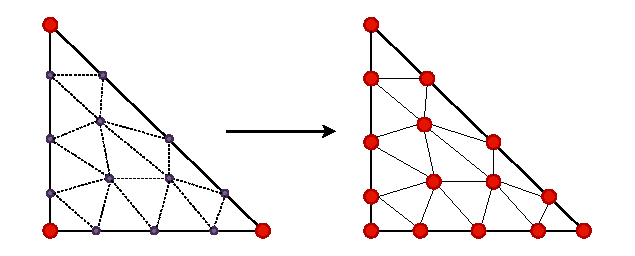
\includegraphics[width=0.5\textwidth]{img/LOR_Triangles.drawio.pdf} % Replace 'example-image.jpg' with the filename of your picture
  \caption{Conceptual representation of the creating the LOR space for triangles. The figure on the right shows the LOR space for a higher order triangular element at \textit{P}=4, which is viewed as a collocated Lagrange basis at \textit{P}=1 on $\mathbf{\xi_{ele}}$ points indicated by red dots. The higher-order element on the left currently shows the nodal expansion basis, which is purely for visualisation.}
  \label{fig:LOR_Triangles}
\end{figure}
The LOR discretisation for triangles requires a different strategy. For a nodal expansion in triangles, that a closed-form expression for Lagrange polynomial does not exist like in the case of tensorial product of modal expansions for Gauss-Lobatto-Legendre (GLL) nodal points. 
Thus, the formation of LOR space, which is always a grid of collocated nodal points, can't be created in a straightforward manner for triangles with either choice of higher-order expansion basis and requires shifting the problem to electrostatic points ($\mathbf{\xi_{ele}}$). 
The problem is interpolated to the LOR space after this shift. The visualisation of the process is seen in Figure ~\ref{fig:LOR_Triangles}, but in reality the construction of the generalised Vandemonde matrix $\mathcal{V}$ takes care of this shift of basis operation.

Tetrahedrons and Prisms follow a similar approach for the construction of the LOR space. 
The visualisation of this construction is seen in Fig.~\ref{fig:LOR_simplices}. Fig.~\ref{subfig:Tet_P3} and ~\ref{subfig:Tet_P6} show the LOR space for tetrahedrons at \textit{P} = 3 and 6. Fig.~\ref{subfig:Prism_P3} and ~\ref{subfig:Prism_P6} show the LOR space for prisms at \textit{P} = 3 and 6, where a prismatic domain expansion is achieved by extending the triangular nodal expansion by making a tensor product with the Lagrange polynomial in the third direction.
\begin{figure}[!htbp]
  \centering
  \begin{subfigure}{0.5\textwidth}
    \centering
    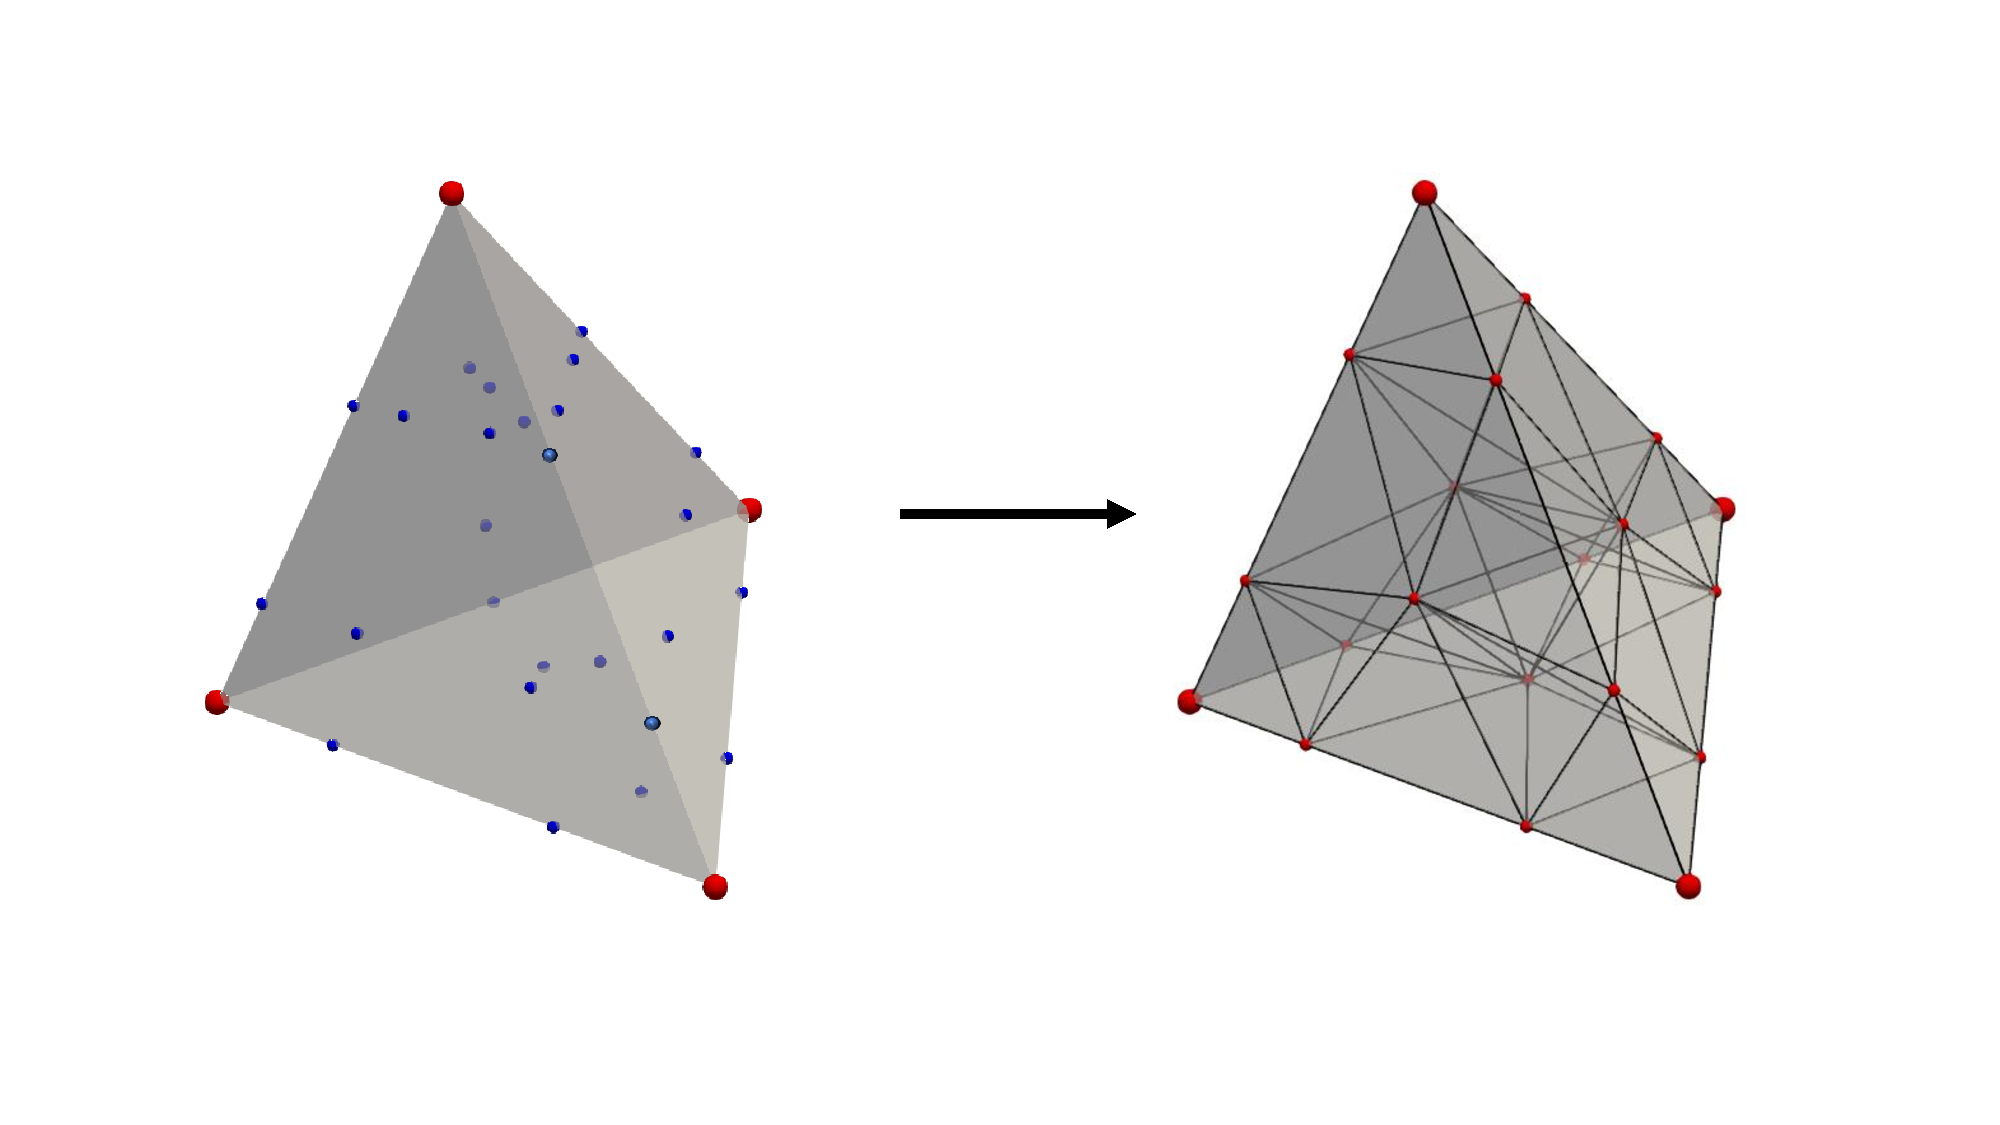
\includegraphics[width=\linewidth]{img/Tet_P3_edit.pdf}
    \caption{Tetrahedron at \textit{P} = 3}
    \label{subfig:Tet_P3}
  \end{subfigure}%
  \begin{subfigure}{.5\textwidth}
    \centering
    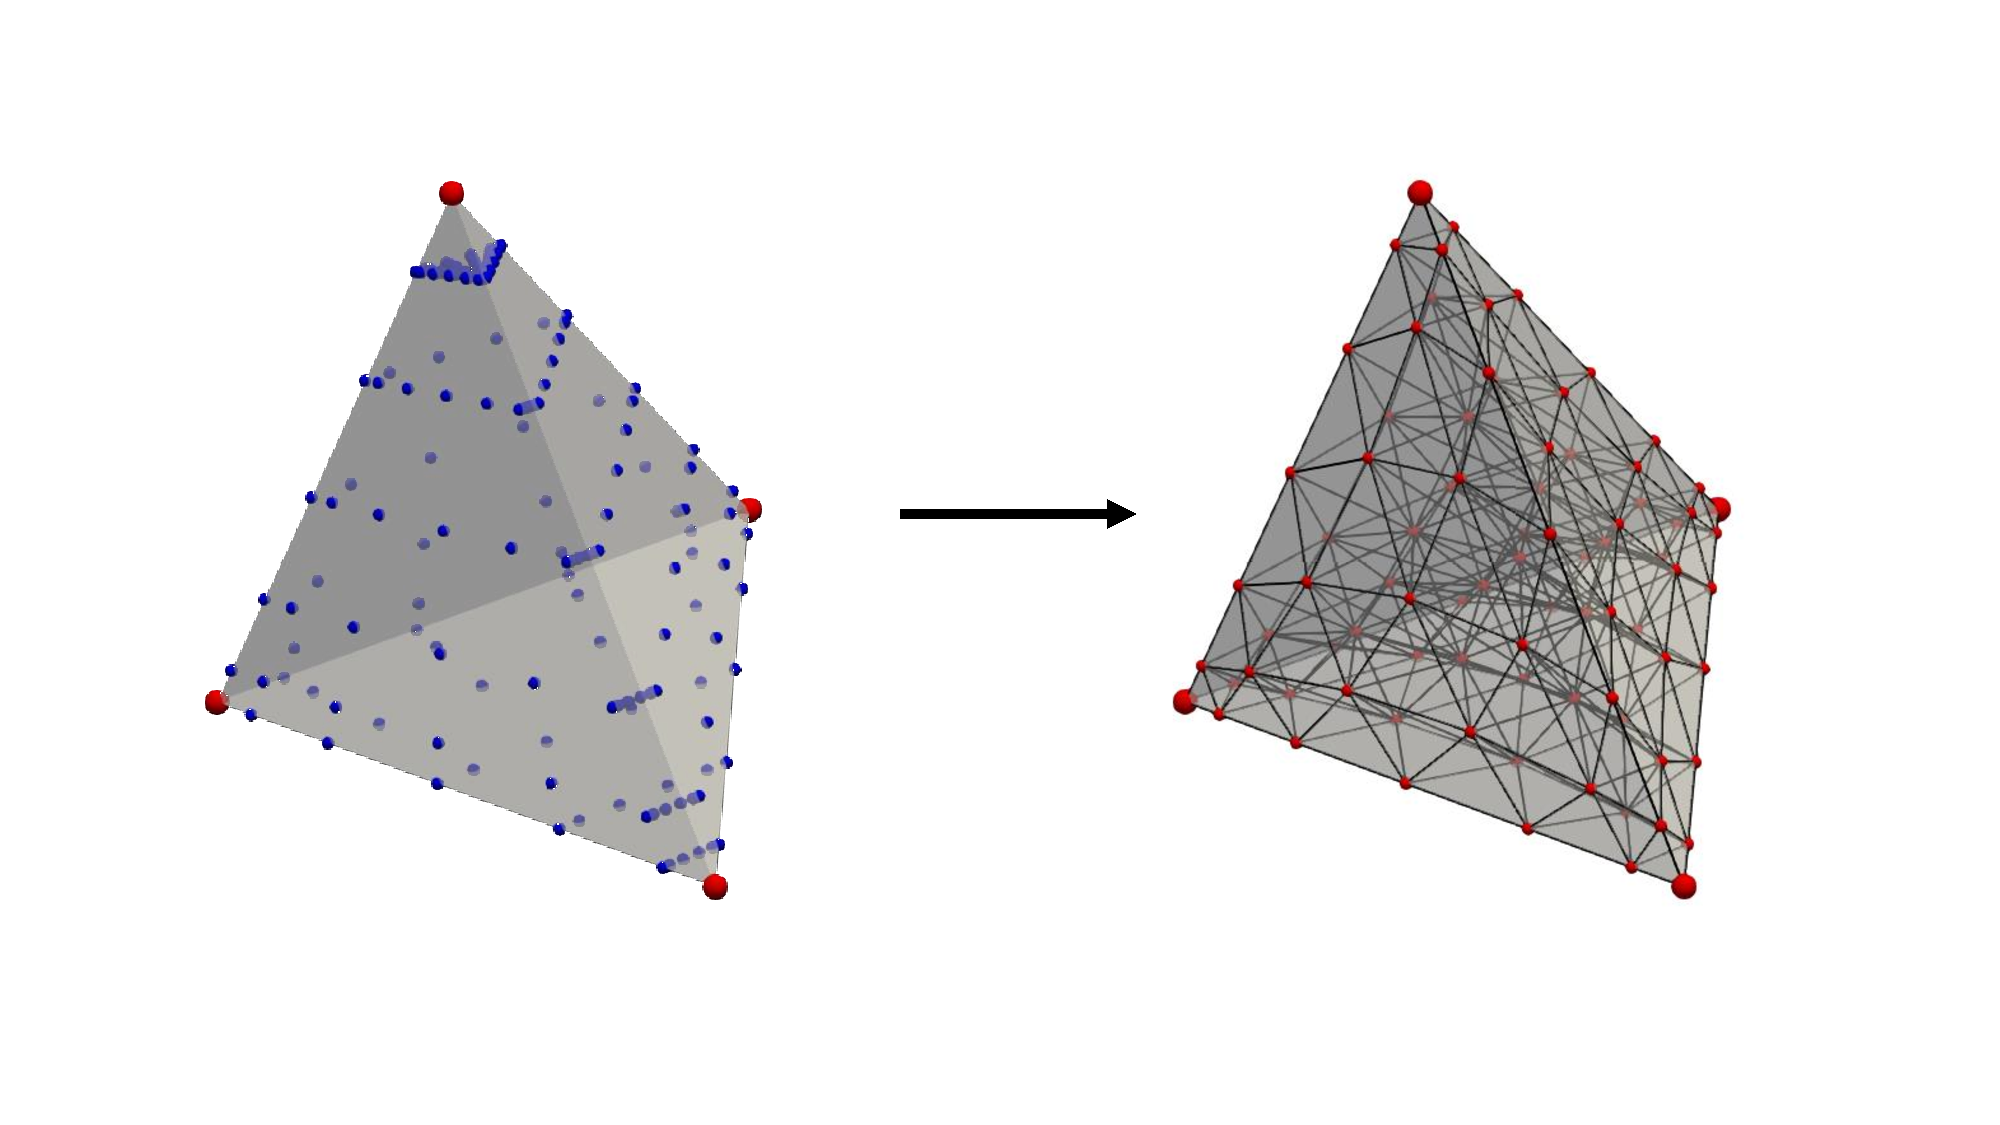
\includegraphics[width=\linewidth]{img/Tet_P6.pdf}
    \caption{Tetrahedron at \textit{P} = 6}
    \label{subfig:Tet_P6}
  \end{subfigure}
  
  \begin{subfigure}{0.5\textwidth}
    \centering
    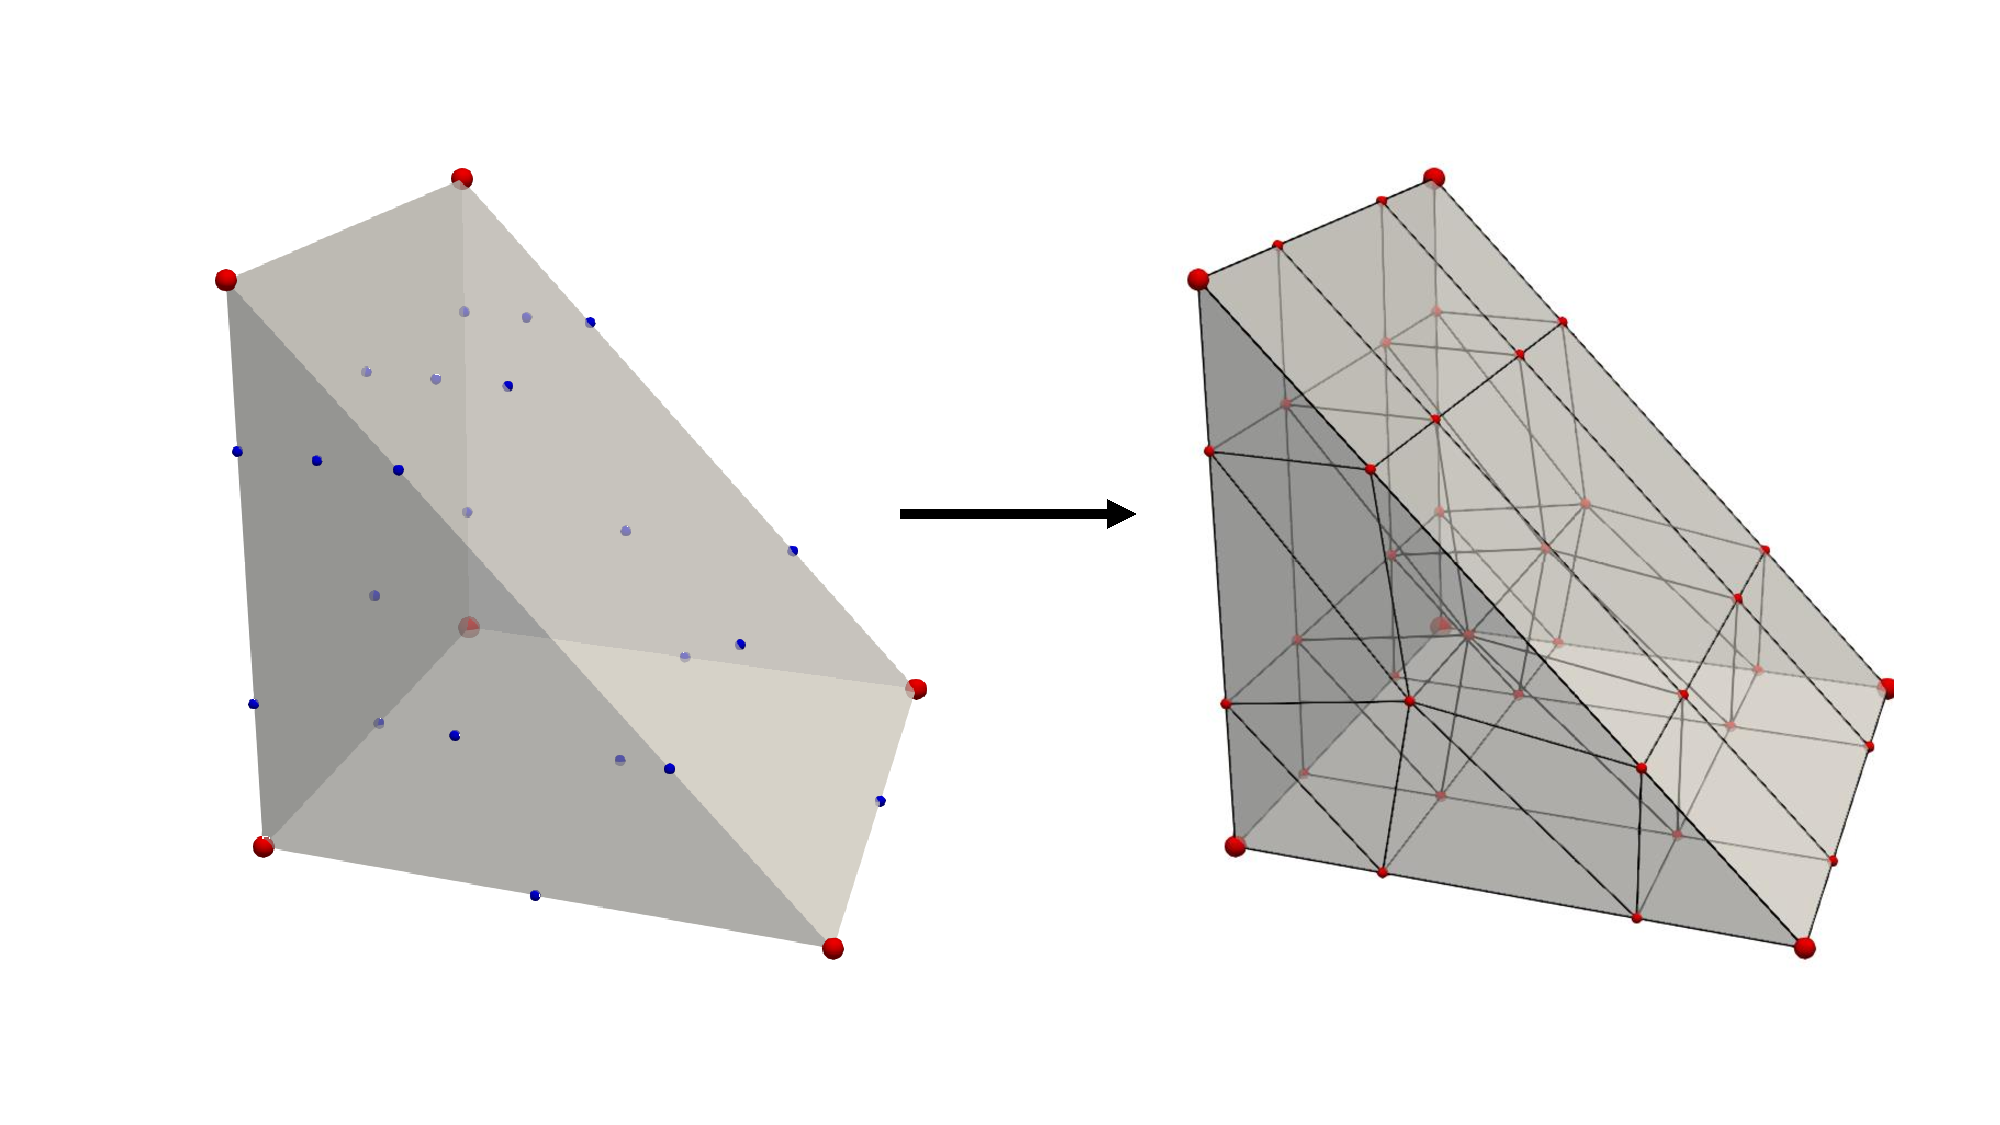
\includegraphics[width=\linewidth]{img/Prism_P3.pdf}
    \caption{Prism at \textit{P} = 3}
    \label{subfig:Prism_P3}
  \end{subfigure}%
  \begin{subfigure}{.5\textwidth}
    \centering
    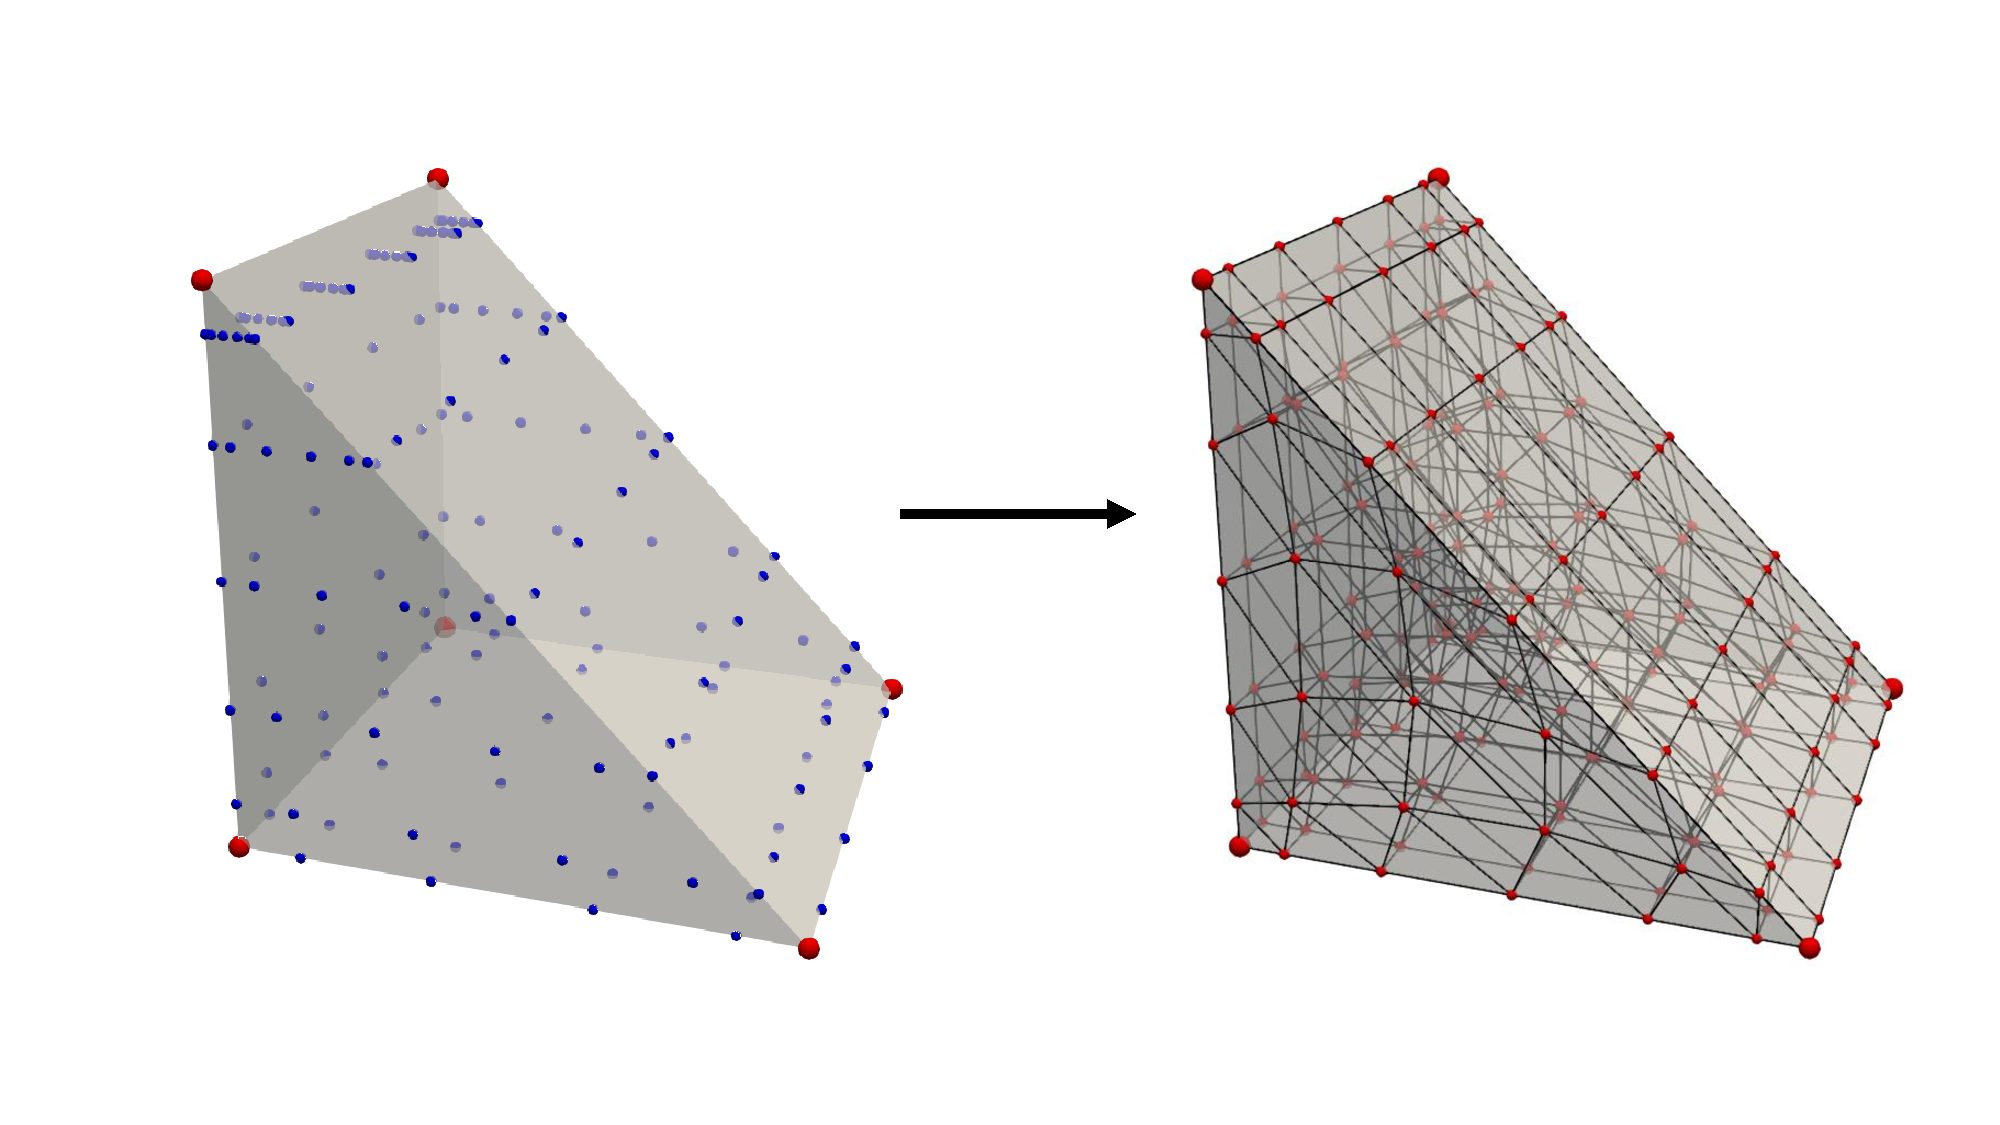
\includegraphics[width=\linewidth]{img/Prism_P6.pdf}
    \caption{Prism at \textit{P} = 6}
    \label{subfig:Prism_P6}
  \end{subfigure}
  \caption{Visual representation of the creating the LOR space for simplices at \textit{P} = 3 and 6. Within each subfigure, the figure on the right shows the LOR space for a HO element on the left. The LOR space is viewed as a collocated Lagrange basis at \textit{P}=1 indicated by red dots, with on $\mathbf{\xi_{ele}}$ points in the interior and $\mathbf{\xi_{GLL}}$ points constrained the boundary. One can identify this by looking at any of the triangular faces for the simplices.}
  \label{fig:LOR_simplices}
  \end{figure}

\subsubsection{LOR setup - Available options}

LOR preconditioner provides various options to setup and solve the preconditioned system. These settings work when the \inltt{GLOBALSYSSOLNINFO} has:
\begin{lstlisting}[style=XMLStyle]
  <I PROPERTY="GlobalSysSoln"             VALUE="IterativeFull" />
  <I PROPERTY="Preconditioner"            VALUE="LOR" />
  <I PROPERTY="LinSysIterSolver"          VALUE="GMRES" />
\end{lstlisting}

The full list is found below:
\begin{lstlisting}[style=XMLStyle]
    <I PROPERTY="GlobalSysSoln"             VALUE="IterativeFull" />
    <I PROPERTY="Preconditioner"            VALUE="LOR"/>
    <I PROPERTY="LinSysIterSolver"          VALUE="GMRES" />
    <I PROPERTY="LORSolverType"             VALUE="DirectFull" />
    <I PROPERTY="LORPointDistribution"      VALUE="GLL" />
    <I PROPERTY="LORSimplex"                VALUE="False" />
\end{lstlisting}

\begin{enumerate}
  \item \inltt{LORSolverType} - The type of solver to use for the inner iteration in the LOR preconditioner, i.e. working on the LOR mesh. most commonly used are \inltt{DirectFull}, \inltt{PETScFull}. Rest are quite experimental, and do not give great performance. They have not been tested extensively in 3D.
  Options:
  \begin{itemize}
      \item \lstinline{DirectFull}: Direct solve on $Ax = b$. Use this with caution when your problem size is greater than 2000 DOF.
      \item \lstinline{XxtFull}: Parallel direct solve on $Ax = b$. Not well tested. 
      \item \lstinline{IterativeFull}: Apply available native linear solvers to solve the LOR system.
      \item \lstinline{Preconditioner}: Option to further apply a preconditioner on the LOR mesh.
  \end{itemize}
  \item \inltt{LORPointDistribution} - Options: \inltt{GLL} (default), \inltt{Equispaced}
  \item \inltt{LORSimplex} - Options: \inltt{True} means $\mathcal{P}1$ type element for quads in the LOR space, \inltt{False} means $\mathcal{Q}1$ type element
\end{enumerate}

The following options are available when \inltt{LORSolverType} = \inltt{IterativeFull}
\begin{enumerate}
  \item \inltt{LORLinSysIterSolver}: Options: All available native linear solvers in Nektar++. Default: \inltt{ConjugateGradient}.
  \item \inltt{LORPreconditioner}: Applying a further preconditioner on the LOR space. Default: \inltt{Diagonal}.
  \item \inltt{LORFixedIterations}: Applying a fixed number of iterations on the \inltt{LORLinSysIterSolver}.
  \item \inltt{LORIterativeTolerance}: The tolerance for the inner loop solver in the LOR preconditioner.
\end{enumerate}
Example:
\begin{lstlisting}[style=XMLStyle]
  <I PROPERTY="LORLinSysIterSolver"    VALUE="GMRES" />
  <I PROPERTY="LORPreconditioner"    VALUE="FullLinearSpace" />
  <I PROPERTY="LORFixedIterations"        VALUE="06" />
  <I PROPERTY="LORIterativeTolerance"      VALUE="1e-4" />
\end{lstlisting}

To use the AMG solver from BoomerAMG to solve the LOR system when \inltt{LORSolverType} = \inltt{PETScFull}, we advise the following settings:

For one V-cycle of BoomerAMG at every iteration (efficient for large 3D cases)
\begin{lstlisting}[style=BashInputStyle]
  -ksp_type preonly
  -pc_type hypre
  -pc_hypre_type boomeramg
  -pc_hypre_boomeramg_max_iter 1
\end{lstlisting}

For applying multiple V-cycles to solve under a certain tolerance (reduces outer iterations, but can be time consuming for large cases)
\begin{lstlisting}[style=BashInputStyle]
  -ksp_rtol 1e-4 #choose your tolerance, keep it high
  -ksp_type richardson
  -pc_type hypre
  -pc_hypre_type boomeramg
\end{lstlisting}

Reliable set of AMG settings for BoomerAMG for non-symmetric Poisson system resulting from LOR discretisation.
\begin{lstlisting}[style=BashInputStyle]
  -pc_hypre_boomeramg_coarsen_type hmis
  -pc_hypre_boomeramg_relax_type_all sor/jacobi
  -pc_hypre_boomeramg_grid_sweeps_all 2
  -pc_hypre_boomeramg_strong_threshold 0.7 #0.25 for 2D cases
  -pc_hypre_boomeramg_interp_type ext+i
  -pc_hypre_boomeramg_P_max 2
  -pc_hypre_boomeramg_truncfactor 0.3
\end{lstlisting}